\chapter{Teaching Your PI Controller to Behave (Part X)}

Throughout this series we have discussed a practical and efficient way to tune the PI controllers in a cascaded velocity loop by simply choosing a factor that determines the desired damping of the system.  From this information, plus a rudimentary knowledge of some of the motor and load parameters, the PI coefficients for the velocity loop and the inner current loops can be calculated.  We developed this technique by first ignoring certain aspects of the control loop, such as the pole of the current controller.  But in blog \ref{ch:6} we reintroduced the current controller’s pole back into the discussion, and evaluated its impact on system performance.

Today, let’s look at the other end of the frequency spectrum.  At low frequencies, viscous damping may affect your velocity loop response times by changing the phase margin at the unity-gain frequency.  When viscous damping is present, it siphons off part of the motor’s torque to do work to move fluid.  Since viscous torque is directly proportional to the speed of the load, we can rewrite the load’s transfer function to be:

\begin{equation}\label{eq:10_1}
    \frac{\omega(s)}{T(s)} = \frac{1}{Js+k_\nu} = \frac{1}{k_\nu \left(\frac{J}{k_\nu}s+1\right)}
\end{equation}
where $k_\nu$ is the viscous damping factor.

As you can see from \ref{eq:10_1}, adding the viscous damping term moves the pole that was at $s = 0$ to $s = k_\nu/J$.  Figure \ref{fig:10_01} shows how the addition of viscous damping changes the load’s Bode plot.

\begin{figure}[H]
    \centering
    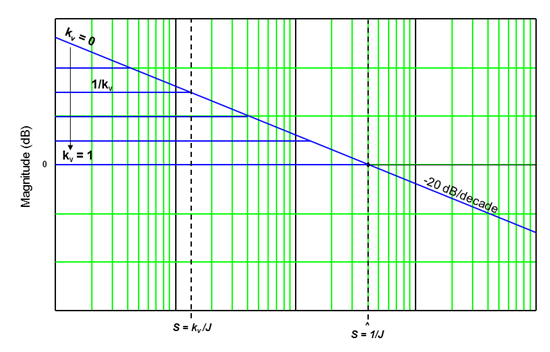
\includegraphics[width=1\linewidth]{10/01}
    \caption{Effect of Viscous Damping ($k_V$) on the Load Bode Plot}
    \label{fig:10_01}
\end{figure}

From Figure \ref{fig:10_01}, we see that as viscous damping increases from zero, low frequency gain plateaus to a value of $1/k_\nu$.  The net effect on the phase plot is to add more phase margin at lower frequencies, since the phase lag of a load with viscous damping will always be less than a load with inertia only.  As a result, stability should actually improve for non-zero values of $k_\nu$.  However, the response time may take a hit, depending on where the velocity open-loop unity-gain frequency is with respect to the pole frequencies shown in Figure \ref{fig:10_01}.  So if your system response is sluggish and the motor doesn’t seem to put out as much torque as it is rated for, you might want to investigate how much viscous damping your system has.

Before closing out this series, I want to address one more important topic.  I have seen and experienced situations myself where the PI coefficients were calculated correctly, but when they were incorporated into the code, the motor either screamed like a banshee or sat there like a lump and did nothing.  So what happened?  In many cases, it was one of the following problems:

\begin{enumerate}
    \item Forgetting to account for the sampling frequency effect on the GAIN of the integrator term.  Figure \ref{fig:10_02} shows how to implement a typical integrator for a digital PI controller.  To scale the output to match what an analog integrator would provide, we must first multiply the input signal by the sampling period “$T$”.  In order to avoid two separate multiply operations, most code examples simply lump $T$ together with the integrator gain term.  If $T$ is not accounted for, you will end up with an integrator gain that is MUCH higher than you anticipated.
    \begin{figure}[H]
        \centering
        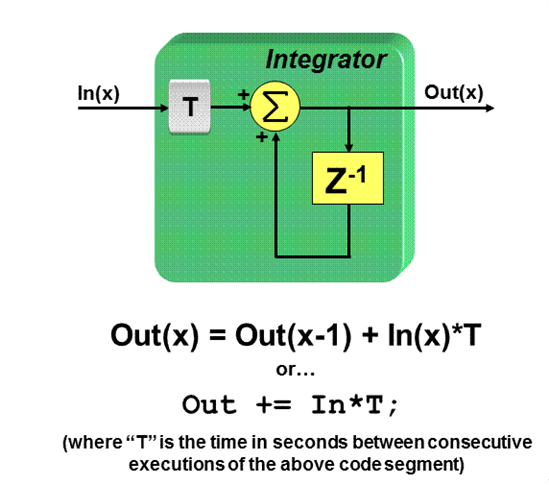
\includegraphics[width=1\linewidth]{10/02}
        \caption{Typical Implementation of a Digital Integrator}
        \label{fig:10_02}
    \end{figure}

    \item So far we have assumed there are no limitations on the number format itself.  If you are using a floating-point processor, then you don’t have to worry about the fractional component of your PI terms.  But most motor control applications are implemented on fixed-point machines for cost reasons.  The good news is that TI has developed a linkable library that is in the ROM of most of our C2000 processors which solves this problem for you.  It is called the “IQ Math” library which stands for “Integer Quotient”.  This allows you to handle floating point values with ease on a fixed-point machine without suffering from the performance hit you typically get with a full-blown floating-point package.  IQ math creates a new variable type in your code which is designated by a “Q” followed by a number.  For example, let’s say you have a 32 bit variable which is typed as a “Q24” variable type.  This means that any variable of this type is assumed to have a 24-bit fractional component, and an 8-bit integer part.  But what occasionally happens is that someone copies TI example code into their design without realizing that our coefficients are represented in IQ format.  For example, if you calculate your I-gain to be \num{10000} (\$00002710 in Q0 format), but you didn’t realize that the TI code assumes the variable is in Q24 format, you will end up with an integrator gain of \num{0.596E-3} instead of \num{10000}.  Obviously, a big difference!  If you make the same mistake for all of the PI coefficients, the motor will most likely just sit there and do nothing since all the gains are way too low.  So, a word to the wise; make sure you know what numerical format your coefficients are represented by.

    \item In some cases, the PI coefficients for an AC Induction Motor drive are calculated correctly and the motor runs just fine\dots until the motor speed exceeds its rated value, at which point the controller response becomes underdamped.  The reason for this can be found back in blog \ref{ch:3} of this series.  The motor transfer function between q-axis current and electromagnetic torque for an AC induction motor is repeated below.
    \begin{equation}
        Mtr(s) = \frac34 P \frac{L_m^2}{L_r}I_d
    \end{equation}

    For speeds up to the rated speed, $I_d$ usually stays constant.  But to achieve speeds beyond the rated speed, you need to reduce the flux in the machine by lowering the value of $I_d$.  You can probably see where I’m going with this.  When you reduce $I_d$, you reduce the gain of the entire velocity loop gain.  If it is reduced too much, you can end up moving the unity-gain frequency to a lower value where the effect of the two poles at $s=0$ have more effect on reducing the phase margin.  To keep the system response from changing, the $K_c$ (or $K_p$) term in the speed PI controller can be increased in direct proportion to the reduction in $I_d$.

    \item Finally, the scaling of the PI coefficients throughout this series has been done assuming we want to represent real system values throughout the signal chain.  For example, the output of the velocity PI controller equals the actual input reference current in amps for the current controller.  The output of the current controller equals the actual voltage applied to the motor winding.  But in many designs, the PI controller outputs are normalized to “Per Unit” (PU) scaling where a value of 1 represents the maximum value possible, and a value of -1 represents the minimum value possible.  For example, a current regulator’s output might be scaled in such a way that 1 corresponds to 100\% PWM, and -1 corresponds to 0\% PWM.  The advantage of this approach is that you can quickly adapt your code to different systems by simply changing your per unit scaling values.  To convert from real-value scaling to PU scaling for $K_a$, $K_b$, $K_c$, and $K_d$ (including the sampling period for the integrators), use the following formulae:

    \begin{equation}
        K_{a\_scaled} = K_a \frac{I_{scale}}{V_{scale}}
    \end{equation}
    where
    \begin{itemize}
        \item $I_{scale}$ is the actual current value corresponding \num{1.0}
        \item $V_{scale}$ is the actual voltage value corresponding to \num{1.0}
    \end{itemize}

    \begin{equation}
        K_{b\_scaled} = K_b T_i
    \end{equation}
    where
    \begin{itemize}
        \item $T_i$ corresponds to the sampling period of the current loop.
    \end{itemize}

    \begin{equation}
        K_{c\_scaled} = K_c \frac{Vel_{scale}}{I_{scale}}\frac{2}{P}
    \end{equation}
    where
    \begin{itemize}
        \item $Vel_{scale}$ = the actual velocity value in \unit{\radian\per\sec} corresponding to \num{1.0}
        \item $I_{scale}$ is the actual current value corresponding \num{1.0}
        \item $P$ = the number of rotor poles on the motor
    \end{itemize}

    \begin{equation}
        K_{d\_scaled} = K_d T_v
    \end{equation}
    where
    \begin{itemize}
        \item $T_v$ corresponds to the sampling period of the velocity loop.
    \end{itemize}

    The PU scaling for traditional parallel PI structures is:
    \begin{align}
        K_{p\_scaled} &= K_{c\_scaled} \\
        K_{i\_scaled} &= K_c K_d \frac{Vel_{scale}}{I_{scale}}\frac{2}{P}T_v
    \end{align}
    where
    \begin{itemize}
        \item $Vel_{scale}$ = the actual velocity value in \unit{\radian\per\sec} corresponding to \num{1.0}
        \item $I_{scale}$ is the actual current value corresponding \num{1.0}
        \item $P$ = the number of rotor poles on the motor
        \item $T_v$ corresponds to the sampling period of the velocity loop.
    \end{itemize}
\end{enumerate}

\textit{\textbf{Note from HA7DN, 2026-04-03:} I am not sure if the VisSim software mentioned here is available today, the supplied link redirects to \url{https://altair.com/embed/}, where a free trial is available, but I have not tried it.}

To assist you with the design of your FOC based speed controller, I have created a VisSim simulation (\href{https://web.archive.org/web/20130813082852/http://e2e.ti.com/group/motor/m/simulations/665001.aspx}{FOC.vsm}) which accepts inputs from an Excel spreadsheet (\href{https://web.archive.org/web/20130813082852/http://e2e.ti.com/group/motor/m/simulations/665002.aspx}{Motor.xlsx}).  If you open the spreadsheet, you can see the parameters for several different motor/load examples as well as the PI controller coefficients which are automatically calculated.  You can also add your own motor and load parameters in the spreadsheet if you want.  To create a \href{https://web.archive.org/web/20130813082852/http://e2e.ti.com/group/motor/m/simulations/665003.aspx}{text output file} which is required by the VisSim simulation, you must perform a “Save As” option, and in the “Save as Type” field, select “CSV (Comma delimited) (*.csv).”  Assuming that this file is in the same folder as "FOC.vsm", you can then open "FOC.vsm" and simply click the run icon on the toolbar at the top of the page to run the simulation.  You can see the speed response (as well as plots of other system variables) by scrolling over to the right side of the simulation window.  The simulation creates a step change in the commanded velocity at $t=0$ which saturates the system, and another step change at $t=\qty{0.5}{\s}$ which doesn’t saturate the system, allowing you to evaluate the system response under both conditions.  If you would like to evaluate another motor /load example, simply double-click on the Motor/Load Selector Block in the bottom-left corner of the simulation window and choose a different option, as shown below.

\begin{figure}[H]
    \centering
    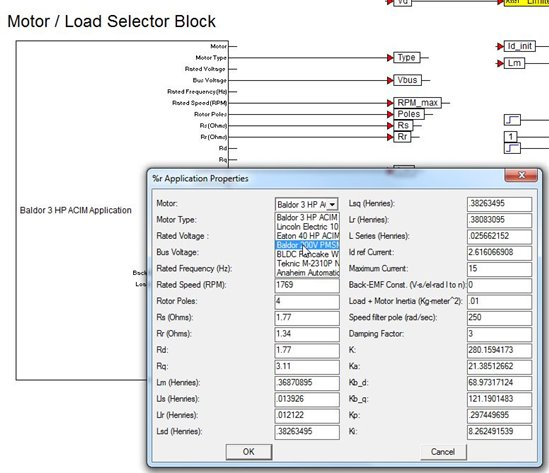
\includegraphics[width=1\linewidth]{10/03}
    \caption{Motor/Load Selector Block in the FOC.vsm Simulation File}
    \label{fig:10_03}
\end{figure}

If you would like to take this simulation out for a test drive, but you don’t have VisSim installed on your machine, simply follow the instructions below:

\begin{enumerate}
    \item Go to Visual Solutions’ \href{https://web.archive.org/web/20130813082852/http://www.vissim.com/}{website}.

    \item In the top right of the browser window, click on “Create account”

    \item After you create an account, click on the “Downloads” tab, and select “VisSim Software”.

    \item Click on the first link on the top of the page that says “VisSim -- Core simulator + UML State Charts + Analyze”

    \item Run the installer program.  This will install the free 60 day trial version of VisSim.
\end{enumerate}

Congratulations\dots we made it!  Thanks for investing your time with me as we have looked at different ways to make your PI control loop behave.  I hope you learned some neat tricks that can help you “stay in tune” with your motor control design.

By the way, if you have suggestions for other motor control topics you would like for me to address in a future blog, I would love to hear from you.  :-)  And of course\dots

Keep Those Motors Spinning,\\

\includegraphics[width=0.2\linewidth]{01/04_dave}\\
\vfill
\textit{May 15 2013 17:13 PM}\\
\url{www.ti.com/motorblog}